%%This is a very basic article template.
%%There is just one section and two subsections.
\documentclass[onehalfspacing]{article}
\usepackage{authblk}
\usepackage{setspace}
\usepackage{titling}
\usepackage{graphicx}
\usepackage{natbib}
\bibpunct{(}{)}{,}{a}{}{;} 
\newcommand{\subtitle}[1]{%
  \posttitle{%
    \par\end{center}
    \begin{center}\large#1\end{center}
    \vskip0.5em}%
}

\begin{document}

\author{Tim Riffe \\ University of California, Berkeley}

\title{A unified model of demographic time}
\subtitle{Paper proposal for the
``Changing patterns of mortality and morbidity: age-, time-, cause- and
cohort-perspectives'' workshop to be held in Prague, 16-18 September, 2015.}

\maketitle


The Lexis diagram relates the age (chronological age), period, and birth cohort
(APC) dimensions of demographic time, but it does not account for remaining years of
life (thanatological age), and its related time indices. The thanatological
counterpart to APC is an identity between thanatological age,
period, and death cohort (TLD). Other identities also exist. For instance,
within a birth cohort (C), chronological age (A), thanatological age (T),
ultimate completed lifespan (L), period (P), and
death cohort (D) are other temporal indices that together redundantly define the
coordinates of a plane (the ATL plane, where P and D are determined by setting
the birth cohort).
Altogether, the relationship between these aspects of time and lifespan can be confusing to any
demographer. These six dimensions have to my knowledge never been considered
jointly. The only subset thereof that has received serious treatment is the APC
framework. Many valid temporal relationships have been neglected outright.

In this paper I first state the relationships between all six dimensions of
demographic time. The APC, TDL, and ATL planes are introduced as degenerate
cases of the unified model. The case of the ATLC cross-sectional plane is
introduced, followed by the full three-dimensional unified model, the APCT
model.
Finally, I demonstrate the use of this coordinate system for the case of
end-of-life trajectories of some characteristics of morbidity. I explain the
utility of this model by demonstrating a case where heterogeneity with respect
to unaccounted-for time dimensions has caused serious misunderstandings in the
scientific literature and in public policy.

\section*{Four planes}

There are at least two ways to think about the model presented here: Either we
situate the model in a ternary 3d space, similar to the tetrahedral simplex, or
we stay in the more familar euclidean 3d space. Since the latter is more
generally intuitive, we opt to describe the intersection of four planes passing
through euclidean space. We begin with the Lexis diagram, and then build out
from there. Two of these four planes motivate the present model, and the other
two are artifacts, with potential demographic meaning.

\subsection*{APC}
The Lexis diagram has long been used in demography to relate chronological age
(A) with birth cohorts (C) and calendar years (P). Since the so-called Lexis
diagram could have been named for others, and since we'll be comparing
with other temporal configurations, let us refer to it as the APC diagram. When
a value (data) is structured by APC coordinates, we refer to it as an APC
surface.

\begin{figure}[ht!]
    \centering
    % figure made in R/LexisStandard.R
    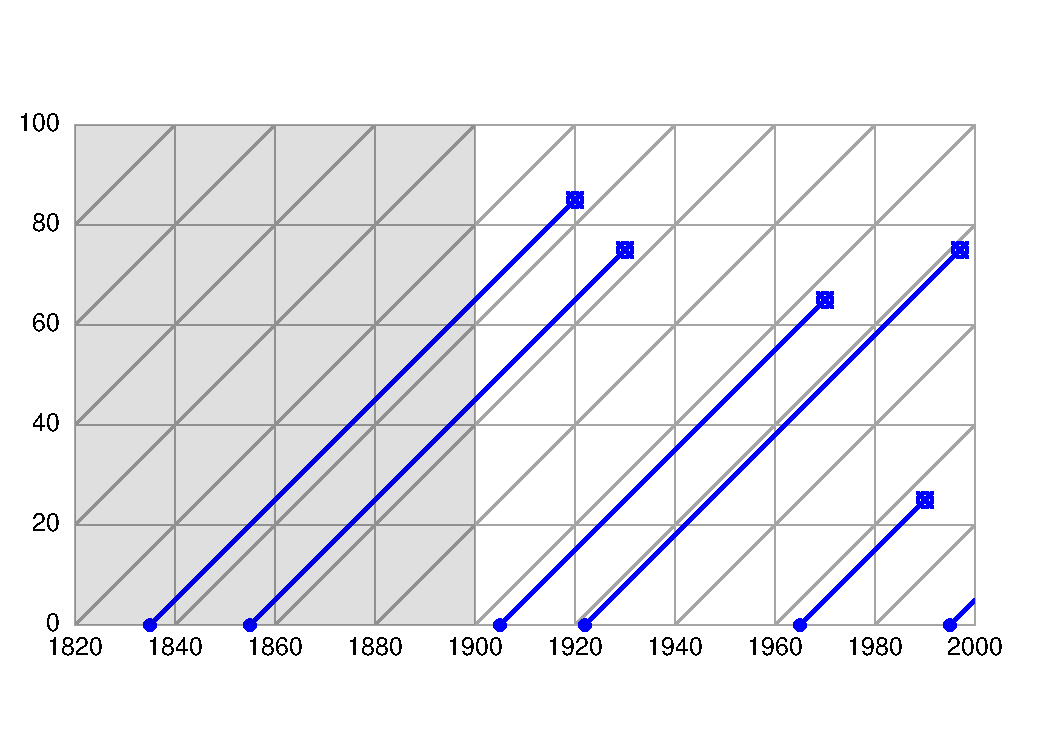
\includegraphics[scale=.7]{Figures/LabPres/APC2.pdf}
    \caption{Lifelines in the APC diagram}
    \label{APCright}
\end{figure} 

Any APC surface can be interpreted along each of these
three dimensions of temporal structure. Such interpretation is a descriptive
task, and it does not succumb to problems of overidentification. Variation along
these three dimensions can not be parsimonsiously separated into effects of A,
P, and C. This is the so-called APC problem, and it is not the concern of the
present work. 




\section*{APCT}
I propose a geometric
identity that unifies all such temporal notions into a single (simple) spatial
relationship that serves as an omnibus conceptual aid to demographers, much as
the Lexis diagram does for APC relationships. The full result is a three
dimensional space that can be disected by any of four different planes,
each of which is parallel to the faces of a regular tetrahedron (see
Figure~\ref{fig:APCT} for a first mock-up of the model).
Each dissecting plane relates three indices of demographic time in proportion to one
another (1:1:1 ternary aspect ratio). The complete space can be described in
geometry nomenclature as the tetrahedral-octahedral honeycomb, which is a kind of space-filling tessellation.\footnote{Constructs following
this geometry exist both in nature and in man-made structures.} 
One of these planes is the familar Lexis plane (horizontal planes in
Figure~\ref{fig:APCT}, and the other three will be new surprises for
demographers. This three dimensional space is not only useful for the sake of formalizing observed temporal relationships, but also for encolosing
demographic time in the past and future (e.g., before the first census and after
the most recent census). 

\begin{figure}[!h]
\centering
\caption[cap]{A mock-up example of the unified model of demographic
time.\footnotemark}
\label{fig:APCT}
	\includegraphics[bb=0 0 3264 2448, width=\textwidth]{Figures/PhysicalModel.jpg}
\end{figure}
\footnotetext{This and other figures to be replaced with vector graphics, although
	I may bring this model to the presentation, since it helps explain concepts.}

A property of the geometry that I propose is that
the time units in every direction (with respect to each index) are proportional. The Lexis
diagram based on right angles and $45^\circ$ birth cohort lines does not have
this property, whereas Lexis diagrams and surfaces based on equilateral
triangles, such as some early proposals \citep[inter
alia, ][]{lexis1875einleitung, lewin1876rapport}, the masterful stereogram of
\citet{perozzo1880della}, or the more recent APC diagram
of \citet{ryder1980cohort}, do have this property. The disecting planes of the
model I propose are likewise composed of equilateral triangles. In Lexis
nomenclature, the 3d projections of an AP square, and AC or PC
parallelograms are all congruent shapes known as regular trigonal trapezohedra
(RTT). The orientation
of a given RTT uniquely defines the Lexis shape in question. Similar constructs
exist in the other time dimensions, and these will also be described. 



\bibliographystyle{plainnat}
  \bibliography{references} 



\end{document}
